\section{Aufgabenmodellierung}

Die Contextual Task Analysis im Usability Engineering Lifecycle dient der Aufgabenanalyse innerhalb der Arbeiten der Benutzer eines Projektes. Nach Mayhew \cite{MD} ist die Analyse der Benutzeraufgaben in den folgenden drei Schritten durchzuführen:
\begin{itemize}
	\item Sammeln von Hintergrundinformationen über die zu automatisierende Arbeit.
	\item Sammeln und Analysieren von Daten aus kontextbezogenen Beobachtungen und Interviews von Benutzern, die in ihrer Arbeitsumgebung arbeiten.
	\item Erstellen des „User Task Organization Model“ anhand der Aufgaben eines Benutzers einer Arbeit.
\end{itemize}

Um Hintergrundinformation über die Arbeit der Benutzer zu erhalten, werden Erkenntnisse aus der Evaluation (s. Anhang: A \nameref{section:Evaluation} ab Seite \pageref{section:Evaluation}) und aus den Dokumentationen (von Journal Stuttgart - RegioTV „Leben mit Diabetes“ und NDR Ratgeber „Typ-2-Diabetes: Wie man vom Insulin wieder wegkommt | Die Ernährungs-Docs | NDR“) die bereits in den Personas verwendet wurden, einbezogen.\newline
In der Aufgabenmodellierung wird zunächst anhand Persona Use Cases und einem Task Scenario die deskreptive Arbeit der Benutzer ohne das zu entwickelnde System analysiert und anschließen durch das Task Organization Model repräsentiert. Um nun eine Aufgabemodellierung hinsichtlich des zu entwickelnden System durchzuführen werden präskriptive Concrete Use Cases, welche die zukünftige Interaktion der Benutzer mit dem System beschreiben, verfasst. 

\subsection{Persona Use Cases (OUC)}

\begin{center}
	\begin{longtable}[H]{|p{2cm}|p{2cm}|p{3cm}|p{3.5cm}|p{2.5cm}|}
		\hline	
		\textbf{Actor} & \textbf{Trigger} & \textbf{Use Case} & \textbf{Task Scenario} & \textbf{Errors,} \\
		\textbf{(User)} &  & \textbf{(Task)} & \textbf{Sequence} & \textbf{Problems, Comments}\\
		\hline	
		Diabetiker & Unwohlge- fühl & OUC 01 Blutzuckerwert messen& 1. Messgerät einschalten und Teststreifen einführen. \newline2. Finger desinfizieren.\newline 3. In den Finger stechen und Blut abtupfen. \newline 4. Blutprobe auf Teststreifen geben. \newline 5. Blutzuckerwert vom Messgerät ablesen.  & Es sollte mindestens 4 mal pro Tag gemessen werden.\newline \newline Alternative Blutgewebemessung mit Sensor.\\
		\cline{2-5}
		& Unter- zuckerung & OUC 02 Unterzuckerung behandeln & 1. Differenz zwischen Blutzuckerwert und Zielwert berechnen. \newline 2. Differenz durch Korreturfaktor teilen, um BE/KE-Anzahl zu erhalten.  \newline  3. BE's/KE's in Form von Einfachzucker essen.& Korrekturfaktor ist indivituell. \newline \newline Bei Unterzuckerung unter 70 mg/dL (4.0 mmol/L) reagieren.\\
		\cline{2-5}
		& Über- zuckerung & OUC 03 Überzuckerung behandeln & 1. Differenz zwischen Blutzuckerwert und Zielwert berechnen. \newline2. Differenz durch Korreturfaktor teilen, um Insulineinheiten zu erhalten. \newline 3. Insulineinheiten spritzen. & Korrektur- faktor  ist indivituell. \newline  \newline Bei Überzuckerung über 180 mg/dL (10.0 mmol/L) reagieren. \\
		\cline{2-5}
		& Hunger & OUC 04 Essen & 1. Mahlzeit wiegen. \newline 2. Kohlenhydrate anhand des Gewichtes der Nahrungsmittel berechnen. \newline  3. Kohlenhydrate in BE/KE umrechnen. \newline 4. BE/KE mit Faktor multiplizieren um Insulineinheiten zu ermitteln. \newline 5. Insulineinheiten spritzen. \newline 6. Spritz-Ess-Abstand einhalten. \newline Essen. & Wenn keine Wage vorhanden, wird geschätzt. \newline \newline Spritz-Ess-Abstand muss eingehalten werden, sonst steigt der Blutzuckerwert bevor das Insulin wirkt.\newline \newline Wenn der Blutzuckerwert vor der Mahlzeit über 250 mg/dL (14.0 mmol/L), darf nicht gegessen werden.\\
		\cline{2-5}
		& Sportliche Bewegung & OUC 05 Sport & 1. Blutzuckermessen. \newline 2. Sport-BE/-KE essen. \newline 3. Alle 20-30 Minuten Blutzucker messen. & Wenn der Blutzuckerwert unter 70 mg/dL (4.0 mmol/L) oder über 250 mg/dL (14.0 mmol/L) kein Sport. \newline \newline Bei Sport ist der Blutzuckerspiegel permanent zu beobachten.\\
		\cline{2-5}
		& Ereignis & OUC 06 Tagebucheintrag erfassen & 1. Uhrzeit eintragen. \newline 2. Blutzuckerwert eintragen. \newline 3. Wenn gegessen, berechnete BE/KE eintragen. \newline 4. Wenn überzuckert, berechnete Korrektureinheiten eintragen. \newline 5. Wenn unterzuckert, berechnete BE/KE eintragen. \newline 6. BE/KE zusammenrechnen und eintragen. \newline 7. Insulineinheiten zusammenrechnen und eintragen. \newline 8. Sporteinheit eintragen. & Nicht bei jedem Ereignis muss alles ausgefüllt werden. \newline \newline Jedes Ereignis muss dokumentiert werden. \newline \newline Täglich sollten 4-8 Ereignisse eingetragen werden.\\
		\hline
		\captionsetup{justification=centering}
		\caption{Persona Use Cases (OCU)}
		\label{tab:Persona Use Cases}
	\end{longtable}
\end{center}

\subsection{Task Scenario}

\begin{center}
	\begin{longtable}[H]{p{2cm}p{12cm}}
		\textbf{Task: }& \textbf{Blutzuckermessung + Mittagessen +  Tagebucheintrag} \\
		 \textbf{User: } & \textbf{Diabetiker}
	\end{longtable}
\end{center}

\textbf{Description: } Dieses Task Scenario umfasst die Behandlung des Diabetes bei dem Verzehr einer Mahlzeit aus 150g Kartoffeln mit 80g Putenfilet. Als Nachtisch wird 50g Vanillepudding serviert. Das Scenario umfasst die Blutzuckermessung, das Berechnen der BE's und Insulineinheiten sowie die anschließende Dokumentation in Form eines Diabetes-Tagebuches.\\
\textbf{Task Flow:}\\
1. Der Diabetiker misst seinen Blutzuckerwert mit einem Messgerät. Dazu trägt er seine Blutprobe aus der Fingerspitze auf dem Teststreifen im Blutzuckermessgerät auf. Der Blutzuckerwert liegt bei 193 mg/dL.\newline
2. Da der Blutzuckerwert 93 mg/dL über dem Zielwert liegt, muss der Diabetiker anhand seines Korrekturfaktors die Korrekturinsulineinheiten berechnen. Der Korrekturfaktor liegt bei 30 mg/dL pro Insulineinheit. Um die Korrekturinsulineinheiten zu ermitteln, dividiert der Diabetiker die 93 mg/dL durch seinen Korrekturfaktor von 30 mg/dL und erhält 3 Korrekturinsulineinheiten.\newline
3. Die Mahlzeit besteht aus Kartoffeln, Putenfilet und Vanillepudding. Da lediglich die Kartoffeln und der Vanillepudding Kohlenhydrate enthalten, muss der Diabetiker anhand der Nährwerttabelle auf den Lebensmittelverpackungen die Kohlenhydrate berechnen. Dazu sind die Kartoffeln und der Pudding separat zu wiegen. Da in 100g Kartoffeln 16g Kohlenhydrate enthalten sind und die Mahlzeit 150g Kartoffeln enthalten, sind die 16g mit 1,5 zu multiplizieren. In 100g Vanillepudding sind 20g Kohlenhydrate und in 50g Pudding 10g Kohlenhydrate enthalten. Insgesamt nimmt der Diabetiker mit dieser Mahlzeit 34g Kohlenhydrate zu sich. \newline
4. Die 34g Kohlenhydrate muss der Diabetiker nun durch 12g teilen um die BE-Anzahl zu erhalten. Somit verzehrt der Diabetiker ca. 3 BE's.\newline
5. Die Anzahl der BE's muss der Diabetiker nun mit seinem BE-Faktor multiplizieren, um die zu spritzenden Insulineinheiten zu erhalten. Da der BE-Faktor des Diabetikers bei 2 liegt, muss dieser für 3 BE's 6 Insulineinheiten spitzen.\newline
6. Diese Insulineinheiten werden mit den Korrektureinheiten addiert und der Diabetiker muss insgesamt 9 Insulineinheiten für seine Mahlzeit spritzen.\newline
7. Nach dem Spritzen der Insulineinheiten muss der Diabetiker 10-15 Minuten mit dem Essen warten, da sonst die Kohlenhydrate den Blutzuckerspiegel schneller ansteigen lässt, als das Insulin wirken kann. \newline
8. Während der Wartezeit trägt der Diabetiker die Daten in sein Diabetes-Tagebuch ein. Zunächst wird die Uhrzeit und der Blutzuckerwert, dann die Korrektureinheiten und BE's und abschließend die gesamten Insulineinheiten notiert.\newline
9. Der Diabetiker beginnt zu essen.
10. Spätestens 2 Stunden nach der Mahlzeit muss eine Kontrollmessung des Blutzuckerspiegels durchgeführt werden. Erst nach 3-4 Stunden verliert das Insulin an Wirkung und der Diabetiker darf, wenn nötig erneut Insulin zur Korrektur spritzen.\\
\textbf{Task Closure: } Dieses Scenario kann beginnt und endet mit dem Messen des Blutzuckerspiegels. Ist der Blutzuckerwert 4 Stunden nach der Mahlzeit in Zielbereich, dauert das Scenario insgesamt 4 Stunden. Ist der Blutzuckerwert allerdings erhöht, verlängert sich das Scenario um weiter 4 Stunden, bis das Korrekturinsulin ebenfalls an Wirkung verliert.\\
\underline{\parbox{\linewidth}{$~$}}
Um den Benutzer bei seiner Aufgabe zu unterstützen sollte das System:
\begin{itemize}
	\item Dem Benutzer die Nährwerte von Lebensmittel aus einer Datenbank ermitteln..
	\item Dem Benutzer das Pflegen einer eigenen Lebensmitteldatenbank ermöglichen.
	\item Dem Benutzer anhand seines Blutzuckers, seiner Faktoren die BE/KE und Insulineinheiten berechnen.
\end{itemize}
Um den Benutzer bei seiner Aufgabe zu unterstützen sollte das user interface:
\begin{itemize}
	\item Dem Benutzer die Eingabe von relevanten Daten des Benutzers ermöglichen.
	\item Dem Benutzer das Dokumentieren von Ereignissen des Benutzers ermöglichen.
	\item Dem Benutzer seine Ereignisse in Form eines Diabetes-Tagebuch repräsentieren.
	\item Dem Benutzer relevante Daten repräsentieren.
\end{itemize}
\underline{\parbox{\linewidth}{$~$}}
\addtocounter{table}{-1}
 \subsection{Task Organization Model}
 Mithilfe der zuvor modellierten deskriptiven Aufgaben soll nach Mayhew ein Task Organization Model erstellt werden \cite{MD}. Die Abbildung \ref{img:taskorganizationmodel}: \nameref{img:taskorganizationmodel}  beschreibt die aktuellen Aufgaben eines Diabetikers ohne System.
 \begin{figure}[H]
 	\centering
 	\setlength{\fboxsep}{1pt}
 	\setlength{\fboxrule}{1pt}
 	\fbox{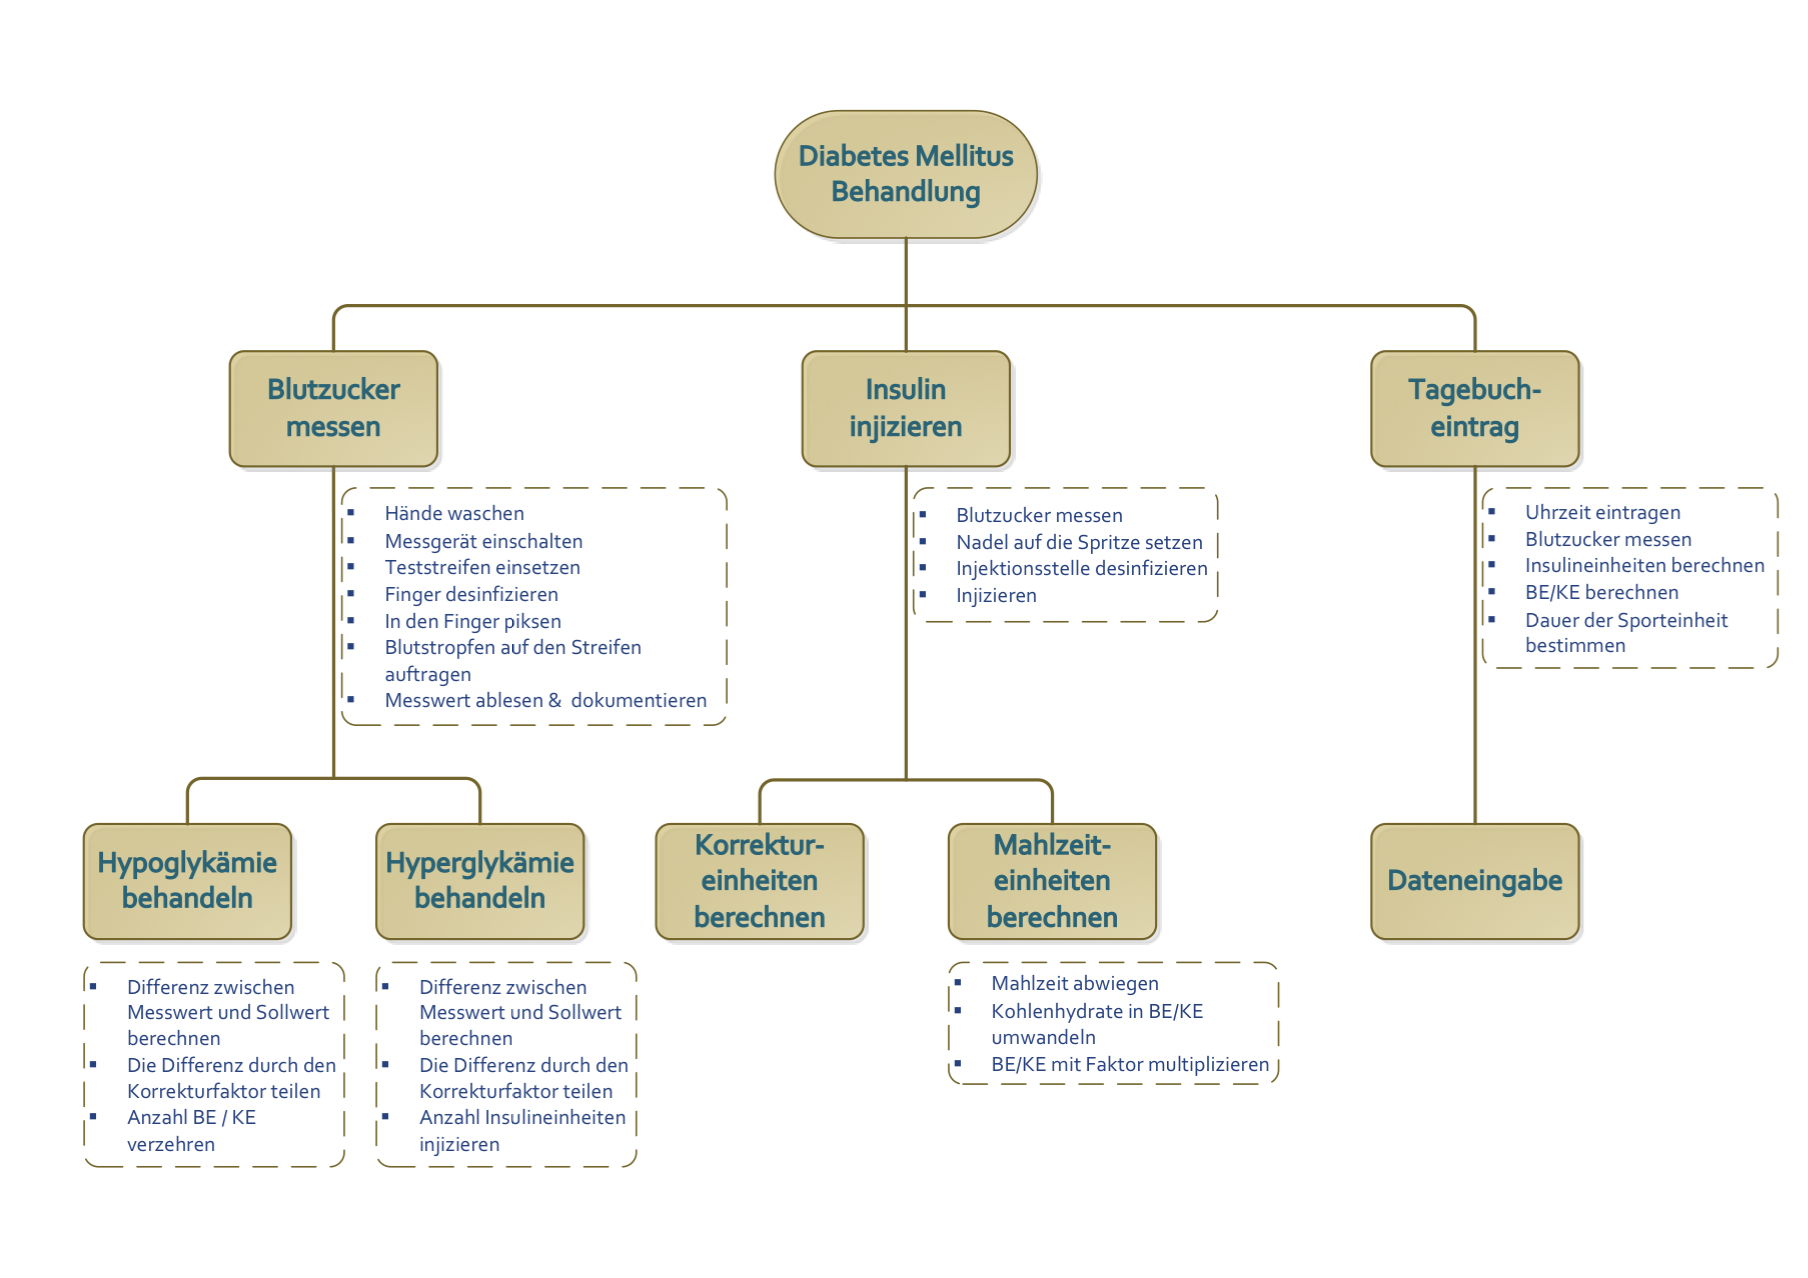
\includegraphics[width=1.0\textwidth]{images/taskOrganizationModel.png}}
 	\captionsetup{justification=centering}
 	\caption{Task Organization Model}
 	\label{img:taskorganizationmodel}
 \end{figure}
 \subsection{Concrete Use Cases (CUC)}
 \paragraph{CUC 01 - Benutzerprofil anlegen}
  \begin{center}
 	\begin{longtable}[H]{|p{6cm}|p{6cm}|}
 		\hline
 		\textbf{User action} & \textbf{System response}\\
 		\hline
 		Der Benutzer möchte ein neues Benutzerprofil anlegen.& Das System präsentiert die Optionen „Anmelden“ und „Registrieren“.\\
 		\hline
 		Der Benutzer wählt die Option „Registrieren“. &  Das System präsentiert ein Formular mit den notwendigen Spezifikationskriterien eines Benutzerprofils.\\
 		\hline
 		Der Benutzer spezifiziert seinen Vornamen, Nachnamen, Geburtsdatum, Geschlecht, Körpergröße, Körpergewicht, Benutzername, 
 		E-Mail-Adresse, Passwort, Behandlungsart, BE/KE-Faktor, Korrekturfaktor, Aktivitäten. & Das System 	füllt das Formular mit den Eingaben.\\
 		\hline
 		Der Benutzer speichert seine Angabe über die Option „Speicher“. & Das System speichert das Benutzerprofil.\\
 		\hline
 		\captionsetup{justification=centering}
 		\caption{CUC 01 - Benutzerprofil anlegen}
 		\label{tab:Persona Use Cases 1}
 	\end{longtable}
 \end{center}
\paragraph{CUC 02 - Benutzerprofil bearbeiten}
\begin{center}
	\begin{longtable}[H]{|p{6cm}|p{6cm}|}
		\hline
		\textbf{User action} & \textbf{System response}\\
		\hline
		Der Benutzer möchte sein bestehendes Benutzerprofil bearbeiten. & Das System präsentiert die Option „Profil bearbeiten“.\\
		\hline
		Der Benutzer wählt die Option „Profil bearbeiten“. &  Das System präsentiert ein Formular und die Spezifikationskriterien des Benutzerprofils.\\
		\hline
		Der Benutzer verändert die Spezifikationskriterien des Benutzerprofils. & Das System nimmt Änderung in das Formular auf.\\
		\hline
		Der Benutzer speichert seine Angabe über die Option „Speicher“. & Das System speichert das Benutzerprofil.\\
		\hline
		\captionsetup{justification=centering}
		\caption{CUC 02 - Benutzerprofil bearbeiten}
		\label{tab:Persona Use Cases 2}
	\end{longtable}
\end{center}
\paragraph{CUC 03 - Diabetes-Ereignis anlegen}
\begin{center}
	\begin{longtable}[H]{|p{6cm}|p{6cm}|}
		\hline
		\textbf{User action} & \textbf{System response}\\
		\hline
		Der Benutzer möchte ein neues Diabetes-Ereignis hinzufügen. & Das System präsentiert die Option „Diabetes“, „Mahlzeit“, „Aktivität“\ und „Beitrag“\\
		\hline
		Der Benutzer wählt die Option „Diabetes“. &  Das System präsentiert ein Formular und die Spezifikationskriterien des Ereignisses mit dem aktuellem Datum und der aktuellen Uhrzeit.\\
		\hline
		Der Benutzer spezifiziert seinen Blutzuckerwert. & Das System nimmt die Eingabe im Formularfeld „Blutzuckerwert" auf und präsentiert im Formularfeld „Korrekturinsulin“ die berechneten Insulineinheiten und im Formularfeld „BE“/„KE“ die berechneten BE/KE.\\
		\hline
		Der Benutzer speichert seine Angabe über die Option „Speicher“. & Das System speichert das Ereignis.\\
		\hline
		\captionsetup{justification=centering}
		\caption{CUC 03 - Diabetes-Ereignis anlegen}
		\label{tab:Persona Use Cases 3}
	\end{longtable}
\end{center}
\paragraph{CUC 04 - Mahlzeit anlegen}
\begin{center}
	\begin{longtable}[H]{|p{6cm}|p{6cm}|}
		\hline
		\textbf{User action} & \textbf{System response}\\
		\hline
		Der Benutzer möchte ein neues Malzeit-Ereignis hinzufügen. & Das System präsentiert die Option „Diabetes“, „Mahlzeit“, „Aktivität“\ und „Beitrag“\\
		\hline
		Der Benutzer wählt die Option „Mahlzeit“. &  Das System präsentiert ein Formular und die Spezifikationskriterien des Ereignisses mit dem aktuellem Datum und der aktuellen Uhrzeit.\\
		\hline
		Der Benutzer spezifiziert die Mahlzeit. & Das System präsentiert eine Auswahlmöglichkeit passender Mahlzeiten.\\
		\hline
		Der Benutzer spezifiziert seine Auwahl. & Das System nimmt die Mahlzeit im Formularfeld „Mahlzeit“ auf.\\
		\hline
		Der Benutzer spezifiziert die Menge der Mahlzeit. & Das System nimmt die Menge im Formularfeld „Menge“ auf, berechnet die BE/KE und Insulineinheiten und präsentiert diese.\\
		\hline
		Der Benutzer speichert seine Angabe über die Option „Speicher“. & Das System speichert das Ereignis.\\
		\hline
		\captionsetup{justification=centering}
		\caption{CUC 04 - Mahlzeit anlegen}
		\label{tab:Persona Use Cases 4}
	\end{longtable}
\end{center}
\paragraph{CUC 05 - Aktivität anlegen}
\begin{center}
	\begin{longtable}[H]{|p{6cm}|p{6cm}|}
		\hline
		\textbf{User action} & \textbf{System response}\\
		\hline
		Der Benutzer möchte ein neues Aktivität-Ereignis hinzufügen. & Das System präsentiert die Option „Diabetes“, „Mahlzeit“, „Aktivität“\ und „Beitrag“\\
		\hline
		Der Benutzer wählt die Option „Aktivität“. &  Das System präsentiert ein Formular und die Spezifikationskriterien des Ereignisses mit dem aktuellem Datum und der aktuellen Uhrzeit.\\
		\hline
		Der Benutzer spezifiziert die Aktivität. & Das System präsentiert eine Auswahlmöglichkeit passender Aktivitäten.\\
		\hline
		Der Benutzer spezifiziert seine Auwahl. & Das System nimmt die Aktivität im Formularfeld „Aktivität“ auf.\\
		\hline
		Der Benutzer spezifiziert die Dauer der Aktivität. & Das System nimmt die Dauer im Formularfeld „Dauer“ auf, berechnet die Kalorien und präsentiert diese.\\
		\hline
		Der Benutzer speichert seine Angabe über die Option „Speicher“. & Das System speichert das Ereignis.\\
		\hline
		\captionsetup{justification=centering}
		\caption{CUC 05 - Aktivität anlegen}
		\label{tab:Persona Use Cases 5}
	\end{longtable}
\end{center}
\paragraph{CUC 06 - Beitrag teilen}
\begin{center}
\begin{longtable}[H]{|p{6cm}|p{6cm}|}
	\hline
	\textbf{User action} & \textbf{System response}\\
	\hline
	Der Benutzer möchte ein neuen Beitrag hinzufügen. & Das System präsentiert die Option „Diabetes“, „Mahlzeit“, „Aktivität“\ und „Beitrag“\\
	\hline
	Der Benutzer wählt die Option „Aktivität“. &  Das System präsentiert ein Eingabefeld für den Inhalt des Beitrages.\\
	\hline
	Der Benutzer spezifiziert den Inhalt des Beitrages. & Das System nimmt die Eingabe auf.\\
	\hline
	Der Benutzer speichert seine Angabe über die Option „Teilen“. & Das System speichert den Beitrag.\\
	\hline
	\captionsetup{justification=centering}
	\caption{CUC 06 - Beitrag teilen}
	\label{tab:Persona Use Cases 6}
\end{longtable}
\end{center}